\chapter{The age of colloidal robots is coming$^{*}$}\footnotetext[1]{Some content in section 1.1 and  section 1.2 of  this  chapter is adapted from " Dou, Y., Dhatt-Gauthier, K., & Bishop, K. J. (2019). Thermodynamic costs of dynamic function in active soft matter. \textit{Current Opinion in Solid State and Materials Science}, 23(1), 28-40." See appendix 4 for the full text of this paper.}
\begin{center}
\vspace*{1\baselineskip}
\textbf{Abstract}
\end{center}
Robotics is in the spotlight of the coming industry 4.0 era \autocite{lasi2014industry}. Highly automatic robots will largely increase productivity and efficiency in many areas such as manufacturing, transportation and retailing. 
It is predicted that 47$\%$ percent of jobs will be replaced by robots in two decades\autocite{frey2017future}.
Research on robotics is related to almost all parts of science and engineering from data science and machine learning to material science and biology. Many developments in robots are inspired by nature to achieve animal or human-like functions. For example,  the famous  bio-inspired robot SPOT$\textregistered$  by Boston Dynamics \autocite{yang2019ten} moves like a four-legged animal to climb stairs and transverse rough terrain with remarkable ease. These and other existing robots are usually in the size of meters. By contrast, this dissertation will focus on the pursuit of robots at micron size typically, 1-100 $\mu m$ (1 $\mu$m = $10^{-6}$ m), the scale of living cells and microorganisms. These colloidal robots are designed to move autonomously through fluid environments to perform programmed tasks of increasing complexity. This chapter introduces the motivation and back ground of the colloidal robots. Then we give a short review of recent research advances on colloidal robots.

\section{Bio-inspired Colloids Robots}
Living cells or microorganism (e.g., bacteria) are the smallest unit of life. Though  only the size of a colloid particle typically from 1 $\mu$m to 100 $\mu$m, living cells can perform  a variety of dynamic characteristic of life. For example, plan cells capture energy from sunlight and convert it into chemical fuels and structural materials; muscle cells powers organisms to move and to transport matter throughout their interiors; the cytoskeleton incessantly reconfigures its structural components, enabling cells to adapt their mechanical properties to their environment; neural cells use complex signaling networks to sense environmental inputs and compute intelligent outputs. Perhaps most remarkably, all cells can grow and replicate to escape the unrelenting pull toward thermodynamic equilibrium (i.e., death).  All of these functions ---and the many others not listed---would be highly desirable to achieve in a small artificial robotics system. 

Inspired by living cells, \textbf{colloidal robots refer to the micron-size machines  dispersed in fluid environments that can perform  programmed autonomous behaviors, such as those found in the living systems including propulsion, navigation, sensing, communication, or even high-level cognition}. Bio-inspired colloids robots are not only trying to mimic dynamics functions in living systems, but also can be engineered to function in extreme environments where living organisms cannot. For example, colloidal robots can be deployed within battery materials for distributed or sensing tasks. From a scientific perspective, the design and synthesis of colloidal robots can deepen our understanding of the non-equilibrium physics that underlies the operation of living systems (e.g., self organization of dissipative structures. See Appendix 4 for a comprehensive review on  synthetic colloids' non-equilibrium physics). Moreover, colloidal robots have promising potential applications in engineering and medical service such as drug delivery\autocite{fu2012controlled,de2017micromotor}, single-cell surgery\autocite{li2017micro}. 

\begin{figure}
\centering
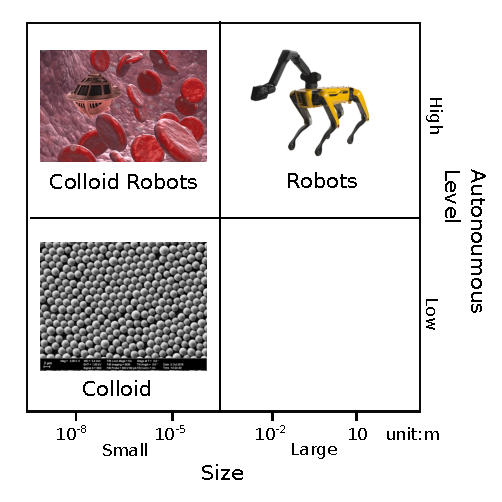
\includegraphics[width=9cm]{figures/1_1.pdf}
\caption{Colloidal robots are the combination of the words "colloid" and "robots". A colloidal robot is in the same size as a colloid particles from $\n m$ to$\mu m$ and usually dispersed throughout the liquid phase. At the same time, a colloidal robot is designed to show dynamics autonomous behaviors such as motion, navigation, and even communication, which are commonly seen in large robotics or living systems.}
\label{fig:1.1}
\end{figure}


\section{Essential Components for Colloidal robots}
Because colloidal robots are still robots, their design shares some of the same basic principles and knowledge from  macroscopic robotic systems.  Traditionally, robots are divided into three essential parts actuators, sensors, and controllers. For example, consider a popular cleaning robot: the Roomba vacuum cleaner (Fig. 1.2).  This robot has two actuator systems: one is responsible for locomotion so that the robot can move around your apartment (wheels); the other is responsible for collecting dust and dirt (brush and vacuum).
The sensors for cleaning robots include infrared  sensors and cameras, which provide information about the environment--for example, the position of obstacles. Using such information, the controllers are programmed  to help cleaning robots plan  the actions. For example, if cleaning robots sense a corner, the controllers will let cleaning robots turn around to avoid crashing. One different thing about controllers is that controllers don't necessarily have physical parts. A controller can be a algorithm or a simple math function.  For all the robots, sensor , actuators, and controllers must work together as a feedback loop so robots can work functionally to finish different task: sensors collect information from the environment; based on information from sensors as well as the target of robots,  controllers will make decisions  on how to move actuators; then the actuators will drive robots into a new environment to repeating this feedback loop. This feedback loop composed of actuators, sensors,  and controllers is also the design guidance to build a colloidal robot. However, due to size limitation and different physics regime of colloidal robots, new mechanisms of actuation, sensing and controlling should be developed compared to the conventional approach in the large scale robots.  In the next section, we will address the challenge to build a colloidal robot. 

\begin{figure}
\centering
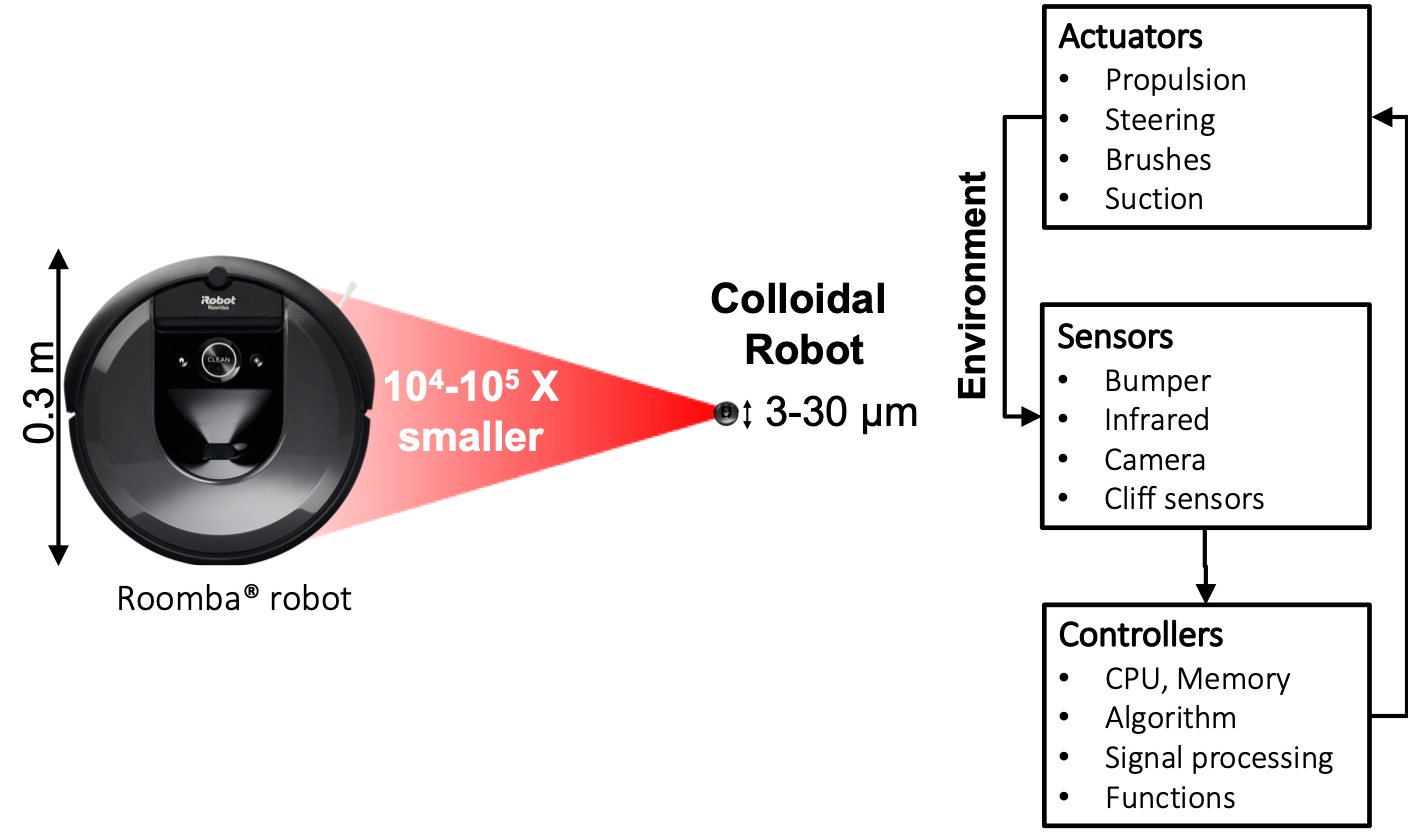
\includegraphics[width=12cm]{figures/1_2.png}
\caption{The essential components and feedback to design a colloidal robot. In the feedback loop, sensors continuously collect information for controllers. Based on  information from sensors and targets of a robot, controllers will make decisions on how to drive the actuators.}
\label{fig:1.2}
\end{figure}

\section{The Challenge to  Build Colloids Robots}

\textbf{Size limitation}. In addition to the three essential components (sensors,actuators, and controllers) introduced above, a robot system also needs power supplies, manipulators with joints and a body frame, etc. For example,  even for a simplest cleaning robot, there are around 100 parts inside. If we simply follow the conventional methods to build a normal size robot, it is not possible to integrate all of these complex components in a micron-size particle (a micron size particle on a cleaning robot is just like a human standing on the earth).  

\textbf{Physics limitation}. Physics for a moving colloid particle in the fluid environment, where everything becomes noisy and sticky, is very different from our normal size world. First, Brownian motions largely affect the motions of colloidal particles, adding stochastic components to the particles' trajectories (Fig. 1.3b shows the diffusion process of Brownian particles). Such thermal motions increase the difficulties in controlling the colloidal robots' accuracy and precision. This requires the actuation mechanism for colloidal robots reliable enough to overcome the background noise. Second, the inertia totally disappears in the small scale as the Reynolds number (Re) of the colloidal robot's system approach to 0.  The Reynolds number (Re) measures the ratio of inertia force and viscosity force represented as
\begin{equation}
    Re=\frac{\rho v l}{\mu}
\end{equation}
where $\rho $ is the density of fluid environment, $v$ is the velocity of the particle, $l$ is the size of particle. $\mu$ is the  viscosity of fluid. In the micron scale, both size and speed of particles are much smaller than 1, leading to the Reynolds number almost 0. The absence of inertia means all of the actuation method in normal size robots based on the reciprocal actuation will no longer work. This interesting  motion restriction in low Reynolds number regime is called Scallop
theory and was first discussed by Edward Purcell\autocite{purcell1977life} (Professor Prucell was famous for his independent discovery of nuclear magnetic resonance, NMR, which brought him a Nobel prize). As shown in Fig. 1.3a, Scallop Theorem states that a swimmer which exhibits time-symmetric motion cannot achieve net displacement in a low Reynolds number fluid environment because all the motion is time reversal. There is no difference between closing a scallop and opening a scallop. New actuation methods for colloidal robots must be designed to break the time-reversal constraint in micron scale. 

\begin{figure}
\centering
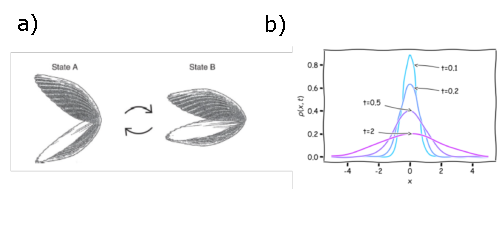
\includegraphics[width=8.5cm]{figures/1_3.pdf}
\caption{Physics challenges for building a colloidal robot (a) Scallop theory: in the micron scale, the effect of inertia almost disappears, making motions time reversal. The reciprocal motions cannot make forward propulsion.  (b) Brownian motion: the presence of thermal noise in the colloid scale let the motion of colloidal robots unpredictable.}
\label{fig:1.3}
\end{figure}
To solve the  challenges mentioned above and design colloidal robots, researchers get inspiration from real small living  machines. The dynamic functions of living cells require integration of structures and processes to drive material organization in space and time. For example in the muscle cells,  the coupling of complex structures (kinesin motor protein) and dissipative processes (ATP hydrolysis) can generate mechanical work (see Fig. 1.4). Thus, a colloidal robot should also have both complex structures and dissipative process. Thanks to the development of nanotechnology, we can now create materials with heterogeneous structure and composition on length scales spanning molecular to macroscopic dimensions with chemical synthesis, lithography, deposition, and etching. These technologies can be directly transplanted to the fabrication process of colloidal robots. In addition to structural and material complexity, the artificial dissipation process for colloidal robots  can be created with chemical reactions, external field (electric, magnetic, acoustic or fluid flow). These non-equilibrium process can generate motions via breaking the time-reversal constraint. For the past decade, lots of research has been conducted to build colloidal robots. Colloidal robotics is now an emerging interdisciplinary field attracting scientists with different background from math, physics to chemistry, biology and engineering. We are goinng to give a state-of-art  review on colloidal robots' research in the next section.
\begin{figure}
\centering
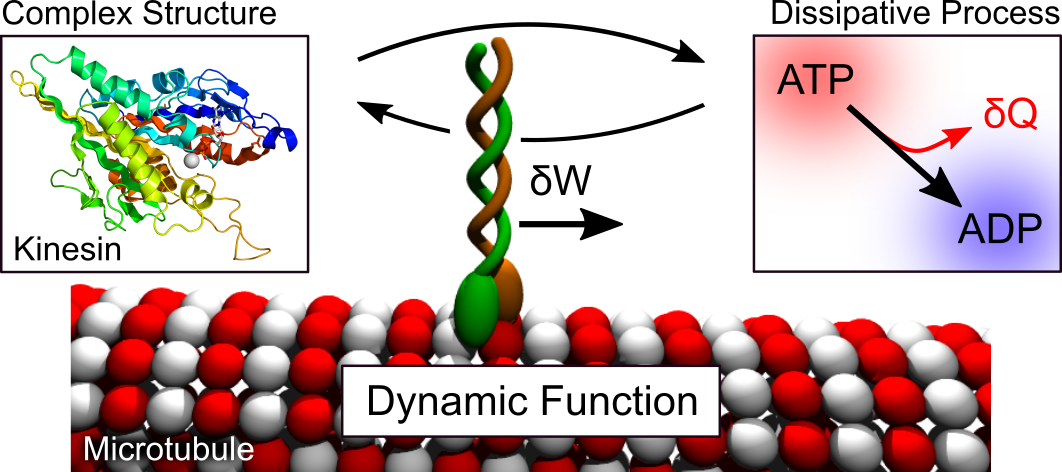
\includegraphics[width=8.5cm]{figures/1_4.png}
\caption{Dynamic functions require the coupling of complex structures and dissipative processes–here, a kinesin motor protein bound to a microtubule  does work powered by ATP hydrolysis.}
\label{fig:1.4}
\end{figure}

\section{A State-of-art Review on Colloidal Robots }
It is not clear which paper first mentioned the similar idea of micron scale robotics (the original concept of  small scale machines can be tracked to Richard Feynman's famous paper, \textit{There's plenty of room at the bottom}\autocite{feynman1960there}). The current research wave in the past decade on the colloidal robots is triggered by the discovery of self propulsion active colloid particles driven by chemical fuels \autocite{paxton2004catalytic}. In 2004, chemists from Pennsylvania State University found that chemical fuels (they use hydrogen peroxide ($H_2O_2$) in the first paper) can drive  gold-platinum bimetallic nanorods' autonomous propulsion. The asymmetric chemical reactions, which happen at the different end of the bimetallic nanorod,  lead to a net flow fluid near the surface of nanorod. This pioneer research then attracted lots of attention in different research field beyond chemistry such as soft condensed matter physics\autocite{Marchetti2013}, materials science\autocite{han2018engineering}, applied math\autocite{fodor2016far} and engineering \autocite{sitti2015biomedical}. More than tens of thousands of papers related to the autonomous behaviors of active colloidal particles have been published since then. However, most of these research papers (either experiment or theory) only focus on building actuators for colloidal robots. Only a few papers show the high autonomous level behaviors in colloidal robots such as navigation or communication\aucite{hong2007chemotaxis,Kline2005}. To the best of our knowledge, the higher level automation behaviors in colloid robots are still challenging, which should be the main research direction in the future. In the following content, we are going to give a short state-of-art review on both experiment approach to colloidal robots as well as some basic theories and simulation methods for colloidal robots. In this short review, we have no intention and interest to rephrase and cover all the research papers on colloidal robots like an encyclopedia book. Instead,  we will focus on the main physics, chemistry and engineering ideas behind these papers. 

\subsection{Experiment Approach}

\textbf{Fabrication.}  High throughput nano/micro scale fabrication technologies in semiconductor manufacturing industry now can make a 3-D structure even smaller than 5 nm \autocite{mokhlesi2010three}. These fancy technologies to make CPU and memory in electronic devices can be transplanted directly to make colloidal robots with almost any desired size, shape and component in cleanroom\autocite{koman2018colloidal}. A typical fabrication process mainly including lithography to make patterns as the main body and frame of colloidal robots, etching to remove unnecessary materials, and deposition to introduce new materials. Multi-layer processing can be designed and optimized to make high dimension and complex structure such as spiral shape\autocite{zhang2009artificial}. After the colloidal robots are fabricated on the wafer, they can be harvested from the silica surface with etching technology or simply physical removal. For the detailed process of fabrication, I would like to direct readers to these three comprehensive reviews\autocite{wong2016synthetic,wang2017emerging, zha2018tubular}. Chemists and material scientists also contributed creative methods to make colloid scale complex structure with one-pot high-throughput chemical synthesis\autocite{youssef2016shape,gong2017patchy,wang2019active}. One challenge for colloidal robots' fabrication is to   make  micron scale soft (or shape-shifting) structure with complex components. Micron scale soft structure  can build colloid robots with high adaptability and flexibility. Liquid crystal, hydrogel gel, droplet, silica polymer, and self-assembled nanoparticles are promising candidate materials for micro/nano scale soft structure \autocite{leong2009tetherless,denkov2015self,zhang2017printing,wei2019molecular}. Another fabrication challenge is to make bio-hybrid colloidal robots,  which can take advantage of  properties in real living systems. Bio-hybrid colloidal robots require high compatibility  among different materials, where experimental biologists can provide invaluable experience and knowledge\autocite{stanton2016biohybrid,magdanz2013development}.

\textbf{Actuation.} Autonomous motion is the most fundamental characteristic of colloidal robots, making colloidal robots real machines instead of simple colloid particles. With designed actuation mechanism, colloidal robots can harness energy from the environment and convert energy into mechanical work. Compared to the inertia driven mechanism in normal size robot, the actuation of colloidal robots always experiencing large hydrodynamics resistance force to balance the driving force. The actuation's power source can be divided into two main categories: chemical/biochemical reactions and the external physical fields. 

Living cells and bacteria use a series of  chemical reaction networks (e.g. ATP hydrolysis) to convert their food source to motions. Colloidal robots can also mimic this type life-like energy conversion mechanism by implementing the chemical reactions on the surface of colloid particles. Such reactions usually happen between the material of colloidal robots and chemical species in the fluid environment. The materials on colloidal robots can work as catalysts or reactants to trigger the reactions in the fluid environment. For example,  colloidal robots,  made of gold or platinum, catalysis the hydrogen peroxide in the fluid to water and oxygen. During the fabrication process, these catalysis or reactant material are patterned at different places of colloidal robots to break the symmetry,  generating chemical species' gradient or reaction product (e.g. bubbles) to actuate colloid particles \autocite{velegol2016origins,shklyaev2016harnessing,parmar2018micro}. Recent reports also showed biochemical reactions (e.g. enzyme) can be options to drive colloidal robot's motions, although the mechanism is still controversial\autocite{zhao2018substrate,somasundar2019positive}.

In addition to  chemical reactions, almost all the external physical fields have been used to powering autonomous motion of colloidal robots including electric fields\autocite{lee2019directed}, magnetic fields\autocite{zhang2009artificial}, acoustic fields\autocite{sabrina2018shape}, lights\autocite{dai2016programmable}, or thermal fields\autocite{lozano2016phototaxis}.  Colloidal robots programmed with physical monopole (e.g. electric point charge), dipole (e.g. magnetic moment), and even quadrupole will respond to the external physical fields, leading to rotation or translation motions. For example, colloidal robots can be fabricated with magnetic materials such as nickel and cobalt to a have magnetic dipole moment. Then an external magnetic field can generate a torque on the colloid's magnetic moment, manipulating the autonomous motion. Compared to the  chemical reaction actuation method, an external physical field can be easily programmed and  drive colloidal robots' motion with less fluctuation\autocite{han2018engineering,ren2018two}. 
The biggest issue in current actuation mechanisms is the very low energy efficiency (usually in the order magnitude of $<10^{-5}$ or less). Colloidal robots always dissipate large amounts of heat\autocite{wang2013understanding} during propulsion compared to the real living cells which can perform efficient motion with much less heat dissipation.

\textbf{Coupled actuation.}  In addition to a single colloid particle's actuation,  colloidal robots can also be actuated via many actuators' interaction and coupling similar to the multi-cylinder engines in a car. These coupled actuation behaviors can perform some life-like collective functions seen in birds swarm and fish flock \autocite{wang2015one,ginot2018aggregation}. Emergent patterns, dynamic clustering, and phase separation have been observed  in different active colloidal particles systems \autocite{buttinoni2013dynamical,ginot2018aggregation,duan2013transition,theurkauff2012dynamic}. The interactions among active colloidal particles are usually in two forms: one is the pure force interaction with each other--for example, charged colloidal particles have electrostatics interactions\autocite{dou2018emergence}; the other is indirect influence--for example, one colloidal particle's motion  will have an influence on the fluid environment, then  the fluid environment will exert this influence back to other colloidal particles in the same environment. Most forms of the second type interaction are hydrodynamic interactions or chemical reactions. For example, the hydrodynamics flow induced by one colloidal particles will attract or repel other colloidal robots from it \autocite{karani2019tuning}. Although active colloidal particles showing collective behaviors can interact with each other, this kind of communication and interaction is still passive and lack of programming. Active colloidal particles cannot take pre-programmed actions from controllers for some desired tasks when they are exerted on some interactions--most papers studying collective behaviors of colloidal robots only observe the phenomena instead of  programming the dynamics.  As a comparison, in normal size robots research, distributed robotics or  swarms robotics\autocite{wei2010sambot,arvin2014colias} can also show life-like dynamics behaviors, but they are more programmable. These robots can communicate with the electronic signal instead of pure physics force. They can not only interact with each other, but also perform programmed reactions and different tasks\autocite{rubenstein2012kilobot,rubenstein2014programmable,li2019particle}.

\textbf{Navigation.} All the living cells or bacteria can sense the information from the environment to navigate themselves for energy, food, or suitable living place. This type of autonomous navigation behaviors is called \textit{-taxis} such as chemotaxis and thermotaxis. Autonomous colloidal robots should be capable of the same kind of navigation abilities. Not so many experiments have been showed to demonstrate  artificial taxis in colloidal robots compared the large amounts of papers on simply showing autonomous motions. Current approaches mainly belong to two mechanisms: the computational vision feedback system and the physical force "correction" method. The computational vision feedback system uses a microscope with digital camera to track the location and velocity of colloidal robots online with a computer vision algorithm. Then based on the information of location, speed of colloid particles, and the desired navigation direction, the computer (controllers) will compute the optimal external field which should be applied in the next time point. This "tracking-computing-applying new field" feedback loop will repeat again and again until colloidal robots reach the destination\autocite{li2017autonomous,han2017sequence}. However, this method has considerable defects. The first disadvantage is the size of the whole system. The navigation behaviors have to be coupled with large complex external devices (microscope, camera, computer, etc.) which is not portable and convenient. Second, this mechanism cannot apply to a large number of colloidal robots with different location and velocity because the external physical field can only satisfy one particle's navigation requirement. 

The second  navigation mechanism, physical force "correction" method, can navigate  colloid to transport following  some gradient information mimicking a living taxis behavior. This method uses the local gradient information (e.g.light intensity, chemical species concentration, temperature) and asymmetric geometry of colloidal particles to generate torque, rotating  the colloidal robot. Such rotation motions will "correct" colloid robots' orientation aligning with the gradient. Then the colloidal robot can move along with gradient in the environment showing navigation behaviors\autocite{brosseau2019relating,ten2014gravitaxis,lozano2016phototaxis,baker2019fight}. However the physical force correction method  lacks the robotic feedback systems with controller and sensors. With this mechanism, a colloid particle cannot navigate itself in a weak gradient environment, where the local stimuli are uniform. Moreover, a colloid particle can only be navigated into one direction with physical "correction" method, which can't be easily re-programmed for doing other types of navigation tasks in a different environments. All of the problems happened to the current approach to autonomous navigation mentioned above are due to the lack of sensors and controllers in the micron scale for colloidal robots.





\subsection{Theory and Simulation}
Richard Feynman said \textit{"What I cannot create, I do not understand."} to emphasize the importance of fundamental understanding of science. This senescence is also true for the  research in colloidal robots. To design a colloidal robot of higher automation level, understanding the physics and mathematics behind colloid robots is as  important as  experimental attempts. Colloidal robots are operated far from the equilibrium state with constant energy and mass flow. Recently years there has been intensively research on non-equilibrium matter, called active matter, in the community of soft matter and statistic physics. Some studies are focusing on building a generally high-level theoretical physics framework for active matter with continuum mechanics or statistical mechanism \autocite{stenhammar2013continuum,solon2015pressure,fodor2016far}. Lots of papers are also trying to use simulation or toy models to discover and design new dynamics behaviors in colloidal robots \autocite{bechinger2016active,speck2014effective,ten2011brownian}. In this section,  basic physical features and mathematical descriptions are going to be reviewed for colloidal robots.  Deeper and detailed derivation can be referred to our citations.

\textbf{Brownian motion.} Colloidal robots' motion is influenced by the thermal noise (Brownian motion) in the fluid environment because of their small size. The Brownian motion can be described with Einstein–Smoluchowski Diffusion Equation\autocite{islam2004einstein}. If we take the colloidal robot as  a rigid spherical body, the translation and rotation diffusion coefficients are,

\begin{equation}
    D_T=\frac{k_B T}{6 \pi \eta R }
\end{equation}
\begin{equation}
    D_R=\frac{k_B T}{6 \pi \eta R^3 }
\end{equation}
where $k_B$ is the Boltzmann constant, $T$ is temperature of the environment, and $\eta$ is the viscosity of fluid, $R$ is the radius of colloidal robots. The diffusion characteristic time is the 
reciprocal of diffusion coefficient, as  $\tau=D^{-1}$. As the size of colloidal robots decrease, the rational diffusion coefficients$D_T$ increase much faster than transnational diffusion coefficients$D_R$. For an actuated colloid with autonomous motion velocity as $v$ in two dimensions, the dynamics can be described as,

\begin{equation}
    \frac{dx}{dt}=v Cos(\theta)+\sqrt{2 D_T}\xi_x, \quad \frac{dy}{dt}=v Sin(\theta)+\sqrt{2 D_T}\xi_y,\quad
    \frac{\theta}{dt}=\sqrt{2 D_R}\xi_\theta
\end{equation}
where $\xi$ is the independent noise with mean as $0$ and correlation as $\delta(t)$. In chemical engineering, we use the Péclet number to represent the dimensionless ratio between convection  and diffusion. For colloidal robots, the Péclet is, 
\begin{equation}
    Pe\propto\frac{v}{\sqrt{D_T D_R}}
\end{equation}
to characterize the influence of Brownian motion on the actuated autonomous motion.

\textbf{Actuated force.} As introduced in the previous section, actuation mechanisms are divided into chemical reactions and physical field actuation. For the chemical reactions driven colloidal robots, the phoretic interaction  model describes the system very well\autocite{golestanian2007,najafi2004simple,golestanian2005propulsion,golestanian2019phoretic}. In this model, the reaction rates are considered much faster than the diffusion rate of chemical species, resulting in the following   
quasi-stationary reaction-diffusion equation,
\begin{equation}
    -D\nabla^2 C=0
\end{equation}
where D is the diffusion coefficient of reactant, this is the Laplace equation for concentration in the fluid environment. The boundary condition for this Laplace equation is  colloidal robots' consuming or producing chemical species as,
\begin{equation}
    -D \texbf{n}\cdot \nabla C|_{r=r_s}=\alpha(r_s)
\end{equation}
where $r$ is the distance from the center of colloid, $r_s$ is the radius of colloid, \texbf{n} is the normal vector on the surface of colloid and $\alpha(r_s)$ is the flux rate. The chemical reaction will lead to a net normal flux(denoted as $\alpha(r_s)$ ) on the surface of colloid. The fluid will response to the local gradient change near the colloids and generate a slip velocity as,
\begin{equation}
    v_s=\mu(r_s)(\textbf{I}-\textbf{n}\textbf{n})\cdot \nabla C(r_s)
\end{equation}
$\mu$ is called mobility measuring the response rate of fluid to the concentration gradient. By making $\alpha$ and $\mu$ positive or negative, the asymmetric chemical activity on the surface can lead to autonomous motion.  Also, both repulsion and attraction forces between colloids can be achieved to study collective behaviors of this system     \autocite{michelin2015autophoretic}.

For the external physical field actuation, the force exerted on each component colloidal robot following the corresponding law of physics. For example, charged colloidal robots with charge amount $q$ experienced electrostatic force $Eq$ in the electric field $E$; magnetic colloid with dipole $m$ in a magnetic field $B$ can be actuated with torque $m\times B$.
Then we can calculate the total force and torque on the rigid body colloidal robots via doing the surface integration if the force is exerted on the surface,
\begin{equation}
    F=\oint_S f_e \,dS
\end{equation}
\begin{equation}
    T=\oint_S (x-x_c)\times f_e \,dS
\end{equation}
where $f_e$  is the component of the actuated force and $x_c$ is the center of colloidal robots.

\textbf{Hydrodynamics.}  The in-compressible viscous fluids are governed by Navier–Stokes equations without any inertia component as discussed in the previous section,
\begin{equation}
    \eta \nabla^2\textbf{u}-\nabla p=0,\quad \nabla \cdot u=0
\end{equation}
where $\eta$ is the viscosity, p is the pressure from fluid. Although hydrodynamic problems are the most complex ones in modeling colloidal robots because of non-linear terms, it is also the most interesting modeling research part with lost of  nontrivial and unexpected results and patterns \autocite{Lauga2009,berke2008hydrodynamic,lauga2011life}. In the low Reynolds number regime, the hydrodynamic force will balance the external force generated by the actuation mechanism. Stokesian dynamics are used to calculate the  translation and angular velocity of colloidal robots \autocite{Brady1988a,Kim2005},
\begin{equation}
    \left[ \begin{array}{c} F \\ T \end{array} \right] = \begin{bmatrix} A & B \\ B^T & C \end{bmatrix} \left[ \begin{array}{c} v \\ \omega \end{array} \right]
\end{equation}
where \textbf{A}, \textbf{B}, and \textbf{C} are tensors determined only by the shape and orientation of the colloidal robots. The whole big matrix is called resistance tensor, which can be calculated analytically\autocite{Kim2005}  Tensor \textbf{B} is called coupling tensor to couple the transition and rotation together. Resistance tensor is no longer symmetric if boundary exists in the fluid environment.  Stokesian dynamics  can be extended to calculate the hydrodynamics interactions between each other via Faxen's law,
\begin{equation}
    F_{drag}=6 \pi \eta a((1+\frac{a^2}{6}\nabla^2)v_{\infty}(0)-U)
\end{equation}
where $F$ is the   force exerted by the fluid on the colloid particles, $a$ is the size of colloid, $u$ is the  the translation  velocity of the colloid and $v$ is the disturbance velocity caused by the presence of other colloids in the fluid environment. We would rather direct our readers to James Swan's paper for the full expression of hydrodynamic interaction in the form of Stokesian dynamics\autocite{swan2011modeling}. Basically, the simulation of colloidal robots' dynamics are solving partial differential equations either numerically or analytically with the physical model showed above. In addition to some commercial multiphysics simulation software such as COMSOL\textregistered, there are also some open-access library written in various coding languages  can help to simulate the dynamics of colloidal robots \autocite{glaser2015strong,anderson2008general,swan2011modeling,singh2019hydrodynamic}.

\textbf{Design and optimization.} For engineering purposes, colloidal robots should be designed with desired functions\autocite{liebchen2019optimal}. As shown in Fig. 1.6, the design process should start with constructing and understanding the design parameters space. For example, how many physics variables (e.g size, temperature, fluid viscosity, choice of materials) should be added into our design space. And then we  need to reduce the dimensions of the design space based on physics and mathematics to make the design problems easier. Dimension reduction is a very essential part of the colloidal robots' design problem. A good dimension reduction will significantly reduce the time used to search for the optimized result. Then we build a physical model to link these design parameters and our target functions of colloidal robots together. This physical model should be adequate enough  to capture all the key physics affecting the dynamics of colloidal robots. At the same time, this model should be concise enough to eliminate unnecessary computation work. After the forward modeling is constructed, we can reverse design the parameter of colloidal robots by defining the desired performance functions such as the highest velocity, or lowest efficiency. Then the final step is to use an optimization algorithm to find the optimal parameters in the design space for the reverse problems \autocite{ward1963hierarchical,nocedal2006numerical}. Recent research also shows that machine learning technology can assist to design colloidal robots with impressive efficiency\autocite{yang2020micro,yang2020cargo,yang2019deep,tsang2018self}.
\begin{figure}
\centering
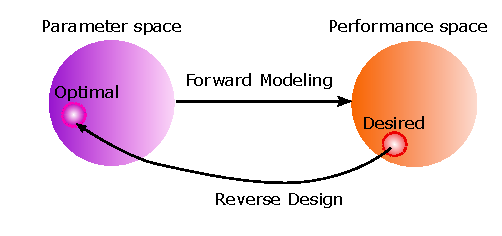
\includegraphics[width=8.5cm]{figures/1_6.pdf}
\caption{The forward modeling connects the design space and performance of colloidal robots together. With the reverse design, the optimal parameters to build a colloidal robot with the desired function can be found.}
\label{fig:1.6}
\end{figure}


%\textbf{Potential Application }
